\documentclass[twoside]{book}

% Packages required by doxygen
\usepackage{fixltx2e}
\usepackage{calc}
\usepackage{doxygen}
\usepackage[export]{adjustbox} % also loads graphicx
\usepackage{graphicx}
\usepackage[utf8]{inputenc}
\usepackage{makeidx}
\usepackage{multicol}
\usepackage{multirow}
\PassOptionsToPackage{warn}{textcomp}
\usepackage{textcomp}
\usepackage[nointegrals]{wasysym}
\usepackage[table]{xcolor}

% Font selection
\usepackage[T1]{fontenc}
\usepackage[scaled=.90]{helvet}
\usepackage{courier}
\usepackage{amssymb}
\usepackage{sectsty}
\renewcommand{\familydefault}{\sfdefault}
\allsectionsfont{%
  \fontseries{bc}\selectfont%
  \color{darkgray}%
}
\renewcommand{\DoxyLabelFont}{%
  \fontseries{bc}\selectfont%
  \color{darkgray}%
}
\newcommand{\+}{\discretionary{\mbox{\scriptsize$\hookleftarrow$}}{}{}}

% Page & text layout
\usepackage{geometry}
\geometry{%
  a4paper,%
  top=2.5cm,%
  bottom=2.5cm,%
  left=2.5cm,%
  right=2.5cm%
}
\tolerance=750
\hfuzz=15pt
\hbadness=750
\setlength{\emergencystretch}{15pt}
\setlength{\parindent}{0cm}
\setlength{\parskip}{3ex plus 2ex minus 2ex}
\makeatletter
\renewcommand{\paragraph}{%
  \@startsection{paragraph}{4}{0ex}{-1.0ex}{1.0ex}{%
    \normalfont\normalsize\bfseries\SS@parafont%
  }%
}
\renewcommand{\subparagraph}{%
  \@startsection{subparagraph}{5}{0ex}{-1.0ex}{1.0ex}{%
    \normalfont\normalsize\bfseries\SS@subparafont%
  }%
}
\makeatother

% Headers & footers
\usepackage{fancyhdr}
\pagestyle{fancyplain}
\fancyhead[LE]{\fancyplain{}{\bfseries\thepage}}
\fancyhead[CE]{\fancyplain{}{}}
\fancyhead[RE]{\fancyplain{}{\bfseries\leftmark}}
\fancyhead[LO]{\fancyplain{}{\bfseries\rightmark}}
\fancyhead[CO]{\fancyplain{}{}}
\fancyhead[RO]{\fancyplain{}{\bfseries\thepage}}
\fancyfoot[LE]{\fancyplain{}{}}
\fancyfoot[CE]{\fancyplain{}{}}
\fancyfoot[RE]{\fancyplain{}{\bfseries\scriptsize Generated by Doxygen }}
\fancyfoot[LO]{\fancyplain{}{\bfseries\scriptsize Generated by Doxygen }}
\fancyfoot[CO]{\fancyplain{}{}}
\fancyfoot[RO]{\fancyplain{}{}}
\renewcommand{\footrulewidth}{0.4pt}
\renewcommand{\chaptermark}[1]{%
  \markboth{#1}{}%
}
\renewcommand{\sectionmark}[1]{%
  \markright{\thesection\ #1}%
}

% Indices & bibliography
\usepackage{natbib}
\usepackage[titles]{tocloft}
\setcounter{tocdepth}{3}
\setcounter{secnumdepth}{5}
\makeindex

% Custom commands
\newcommand{\clearemptydoublepage}{%
  \newpage{\pagestyle{empty}\cleardoublepage}%
}

\usepackage{caption}
\captionsetup{labelsep=space,justification=centering,font={bf},singlelinecheck=off,skip=4pt,position=top}

%===== C O N T E N T S =====

\begin{document}

% Titlepage & ToC
\pagenumbering{alph}
\begin{titlepage}
\vspace*{7cm}
\begin{center}%
{\Large t\+A\+Itris \\[1ex]\large v1.\+0 }\\
\vspace*{1cm}
{\large Generated by Doxygen 1.8.13}\\
\end{center}
\end{titlepage}
\clearemptydoublepage
\pagenumbering{roman}
\tableofcontents
\clearemptydoublepage
\pagenumbering{arabic}

%--- Begin generated contents ---
\chapter{File Index}
\section{File List}
Here is a list of all files with brief descriptions\+:\begin{DoxyCompactList}
\item\contentsline{section}{src/\textbf{ t\+A\+Itris.\+c} \\*Main file }{\pageref{tAItris_8c}}{}
\item\contentsline{section}{src/ai/genetic/\textbf{ core.\+c} \\*Core of the genetic algorithm }{\pageref{core_8c}}{}
\item\contentsline{section}{src/ai/genetic/\textbf{ core.\+h} \\*Core of the genetic algorithm }{\pageref{core_8h}}{}
\item\contentsline{section}{src/ai/genetic/\textbf{ engine.\+c} \\*Engine for the genetic algorithm }{\pageref{engine_8c}}{}
\item\contentsline{section}{src/ai/genetic/\textbf{ engine.\+h} \\*Engine for the genetic algorithm }{\pageref{engine_8h}}{}
\item\contentsline{section}{src/ai/genetic/\textbf{ tools.\+c} \\*Tools for the genetic algorithm }{\pageref{tools_8c}}{}
\item\contentsline{section}{src/ai/genetic/\textbf{ tools.\+h} \\*Tools for the genetic algorithm }{\pageref{tools_8h}}{}
\item\contentsline{section}{src/debug/\textbf{ debug.\+h} \\*Debug }{\pageref{debug_8h}}{}
\item\contentsline{section}{src/debug/engine/\textbf{ debug\+\_\+state.\+c} \\*Debug state }{\pageref{debug__state_8c}}{}
\item\contentsline{section}{src/debug/engine/\textbf{ debug\+\_\+state.\+h} \\*Debug state }{\pageref{debug__state_8h}}{}
\item\contentsline{section}{src/engine/\textbf{ angle.\+h} \\*Angle }{\pageref{angle_8h}}{}
\item\contentsline{section}{src/engine/\textbf{ board.\+c} \\*\doxyref{Board}{p.}{structBoard} }{\pageref{board_8c}}{}
\item\contentsline{section}{src/engine/\textbf{ board.\+h} \\*\doxyref{Board}{p.}{structBoard} }{\pageref{board_8h}}{}
\item\contentsline{section}{src/engine/\textbf{ cell.\+h} \\*Cell }{\pageref{cell_8h}}{}
\item\contentsline{section}{src/engine/\textbf{ input.\+h} \\*Input }{\pageref{input_8h}}{}
\item\contentsline{section}{src/engine/\textbf{ motion.\+c} \\*Motion }{\pageref{motion_8c}}{}
\item\contentsline{section}{src/engine/\textbf{ motion.\+h} \\*Motion }{\pageref{motion_8h}}{}
\item\contentsline{section}{src/engine/\textbf{ score.\+c} \\*Scoring system }{\pageref{score_8c}}{}
\item\contentsline{section}{src/engine/\textbf{ score.\+h} \\*Scoring system }{\pageref{score_8h}}{}
\item\contentsline{section}{src/engine/\textbf{ state.\+c} \\*\doxyref{State}{p.}{structState} }{\pageref{state_8c}}{}
\item\contentsline{section}{src/engine/\textbf{ state.\+h} \\*\doxyref{State}{p.}{structState} }{\pageref{state_8h}}{}
\item\contentsline{section}{src/engine/piece/\textbf{ piece.\+c} \\*\doxyref{Piece}{p.}{structPiece} }{\pageref{piece_8c}}{}
\item\contentsline{section}{src/engine/piece/\textbf{ piece.\+h} \\*\doxyref{Piece}{p.}{structPiece} }{\pageref{piece_8h}}{}
\item\contentsline{section}{src/engine/piece/\textbf{ piece\+\_\+queue.\+c} \\*\doxyref{Piece}{p.}{structPiece} queue }{\pageref{piece__queue_8c}}{}
\item\contentsline{section}{src/engine/piece/\textbf{ piece\+\_\+queue.\+h} \\*\doxyref{Piece}{p.}{structPiece} queue }{\pageref{piece__queue_8h}}{}
\item\contentsline{section}{src/engine/piece/\textbf{ piece\+\_\+shape.\+h} \\*\doxyref{Piece}{p.}{structPiece} shape }{\pageref{piece__shape_8h}}{}
\item\contentsline{section}{src/engine/piece/\textbf{ piece\+\_\+type.\+h} \\*\doxyref{Piece}{p.}{structPiece} type }{\pageref{piece__type_8h}}{}
\item\contentsline{section}{src/engine/piece/\textbf{ seven\+\_\+bag.\+c} \\*7-\/\+Bag generator }{\pageref{seven__bag_8c}}{}
\item\contentsline{section}{src/engine/piece/\textbf{ seven\+\_\+bag.\+h} \\*7-\/\+Bag generator }{\pageref{seven__bag_8h}}{}
\item\contentsline{section}{src/utils/\textbf{ ansi\+\_\+code.\+h} \\*A\+N\+SI escape code }{\pageref{ansi__code_8h}}{}
\item\contentsline{section}{src/utils/\textbf{ random.\+h} \\*Random number generation }{\pageref{random_8h}}{}
\item\contentsline{section}{src/utils/\textbf{ safe\+\_\+op.\+h} \\*Safe operations }{\pageref{safe__op_8h}}{}
\end{DoxyCompactList}

\chapter{File Documentation}
\section{src/t\+A\+Itris.c File Reference}
\label{tAItris_8c}\index{src/t\+A\+Itris.\+c@{src/t\+A\+Itris.\+c}}


Main file.  


{\ttfamily \#include \char`\"{}utils/random.\+h\char`\"{}}\newline
{\ttfamily \#include \char`\"{}engine/piece/piece\+\_\+queue.\+h\char`\"{}}\newline
{\ttfamily \#include \char`\"{}engine/state.\+h\char`\"{}}\newline
{\ttfamily \#include \char`\"{}debug/engine/debug\+\_\+state.\+h\char`\"{}}\newline
Include dependency graph for t\+A\+Itris.\+c\+:
\nopagebreak
\begin{figure}[H]
\begin{center}
\leavevmode
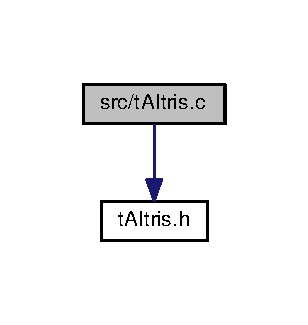
\includegraphics[width=350pt]{tAItris_8c__incl}
\end{center}
\end{figure}
\subsection*{Functions}
\begin{DoxyCompactItemize}
\item 
int \textbf{ main} ()
\end{DoxyCompactItemize}


\subsection{Detailed Description}
Main file. 

\begin{DoxyAuthor}{Author}
S4\+Master\+Race 
\end{DoxyAuthor}
\begin{DoxyVersion}{Version}
2.\+0 
\end{DoxyVersion}


\subsection{Function Documentation}
\mbox{\label{tAItris_8c_ae66f6b31b5ad750f1fe042a706a4e3d4}} 
\index{t\+A\+Itris.\+c@{t\+A\+Itris.\+c}!main@{main}}
\index{main@{main}!t\+A\+Itris.\+c@{t\+A\+Itris.\+c}}
\subsubsection{main()}
{\footnotesize\ttfamily int main (\begin{DoxyParamCaption}{ }\end{DoxyParamCaption})}


%--- End generated contents ---

% Index
\backmatter
\newpage
\phantomsection
\clearemptydoublepage
\addcontentsline{toc}{chapter}{Index}
\printindex

\end{document}
